\documentclass[a4paper,11pt]{jarticle}
%\usepackage{graphicx}% Include figure files
\usepackage[dvipdfmx]{graphicx}
\usepackage{dcolumn}% Align table columns on decimal point
\usepackage{bm}% bold math
\usepackage{amssymb}
\usepackage{amsmath}

\def\vecR {\bm {\mathcal {R} } }
\def\R  {\mathcal {R} }
\pagestyle{plain}
\title{チュートリアル}
\author{牧野真人}
\date{\number\year 年\number\month 月\number\day 日}
\begin{document}
\maketitle
%%%%%%%%%%%%
\section{はじめに}
本文書は(磁石)振り子のプログラムであるPEMのチュートリアルである。
ここでは、2つの例をあげる。
まずは、簡単な例として楕円体の自由回転をシミュレーションする。
そのあと、磁石振り子のシミュレーションを例にする。
このシミュレーションは磁石を持った質点の振り子として文献\cite{doi}にある。
\section{楕円体の自由回転}
\subsection{入力UDF}
中身のないファイルをまず作成する。ファイル名は、任意でもよいが、
\begin{verbatim}
ellipsoid.udf
\end{verbatim}
とする。
拡張子はudfとする。
ファイルをテキストエディタで開き、
\begin{verbatim}
\include {"pem1_3_def.udf"}
\end{verbatim}
と記述して、保存する。
このファイルをGOURMETより開いて編集する。

データ名
\begin{verbatim}
unitParameter
\end{verbatim}
以下には、PEMの単位としている長さ、質量、時間、電流の値をいれる。
今回は、特に入力しないで進める。

\begin{verbatim}
body[]
\end{verbatim}
では、
剛体の情報をいれる。
この後、設定する
\begin{verbatim}
simulation.pendulum[]
\end{verbatim}
\begin{verbatim}
simulation.body[]
\end{verbatim}
では、この\verb|body[]|の\verb|id|を指定して、利用することになる。
まず、要素を一つ増やす。
メニューの\verb|Edit|の\verb|Insert an Array Element|
か\verb|Add an Array Element|、あるいは、
ショートカットキーとして、
ctrl+i、ctrl+eで要素を増やすことが出来る。

要素が増えたら
\begin{verbatim}
body[0].id
\end{verbatim}
に
\begin{verbatim}
0
\end{verbatim}
を入れる。
\verb|id|は他のものと重複しなければ、任意の整数で良い。
\verb|body[]|は複数の\verb|shape[]|から構成する。もちろん一つでも良い。
今回は、一つだけにする。\verb|shape[]|に要素を一つ増やす。
\begin{verbatim}
body[0].shape[0].center.x
body[0].shape[0].center.y
body[0].shape[0].center.z
\end{verbatim}
は、\verb|[0,0,0]|を入れる。
粒子固定座標系での回転の中心が原点であり、この\verb|shape[0]|の中心が回転の中心となる。
この後、入力する楕円体の中心が回転の中心になる。
また、ここで入力している座標は、粒子の固定座標系で$\bm{u}_1,\bm{u}_2,\bm{u}_3$を基底とする座標系を入力していることになる。
\begin{verbatim}
body[0].shape[0].mass
\end{verbatim}
は
\begin{verbatim}
1
\end{verbatim}
とする。
質量を入力した。
\begin{verbatim}
body[0].shape[0].shape
\end{verbatim}
は
\begin{verbatim}
ellipsoid
\end{verbatim}
を選択する。
\begin{verbatim}
body[0].shape[0].ellipsoid.a
body[0].shape[0].ellipsoid.b
body[0].shape[0].ellipsoid.c
\end{verbatim}
には、楕円体の径の長さを指定する。
\begin{verbatim}
body[0].shape[0].ellipsoid.da.x
body[0].shape[0].ellipsoid.da.y
body[0].shape[0].ellipsoid.da.z
\end{verbatim}
および
\begin{verbatim}
body[0].shape[0].ellipsoid.db.x
body[0].shape[0].ellipsoid.db.y
body[0].shape[0].ellipsoid.db.z
\end{verbatim}
には、径$a,b$に相当する単位ベクトルを入れる。
楕円体の3つの軸は直交するため、この2つの外積から、\verb|body[0].shape[0].ellipsoid.dc|に相当するものは計算されるため入力を要求していない。
\begin{verbatim}
body[0].magnet[]
\end{verbatim}
以下には、磁気ダイポール(磁石)の情報をいれるが、ここでは、考えない。
\begin{verbatim}
body[0].color[0].red
body[0].color[0].green
body[0].color[0].blue
body[0].color[0].trans
\end{verbatim}
は、\verb|body[0].shape[0]|に相当する色を赤緑青および透明度を0から1の値を入れる。
また、\verb|body[0].shape[]|の要素数と\verb|body[0].color[]|の要素数が一致しない場合\verb|body[0].color[0]|の色で、
すべての\verb|body[0].shape[]|を\verb|body[0].color[0]|の色で描画する。

\begin{verbatim}
body[0].analysis
\end{verbatim}
以下は、\verb|body[0].shape[]|の値を元に解析した結果が入る。
解析は、データ名
\begin{verbatim}
body[0]
\end{verbatim}
の上を右クリックして、actionのメニューを出して
\begin{verbatim}
analyzer
\end{verbatim}
をクリックして解析する。
この場合は、\verb|body[0]|のみを解析するが、
\begin{verbatim}
analyzer_all
\end{verbatim}
をクリックすると、すべての\verb|body[]|を解析する。

\begin{verbatim}
body[0]
\end{verbatim}
の形状、磁気ダイポールをプロットするには、
actionの
\begin{verbatim}
show....
\end{verbatim}
を選択すれば良い。

この\verb|body[0]|を配置して、シミュレーションを行う。
\begin{verbatim}
simulation.time.simulationSteps
simulation.time.reportSteps
simulation.time.dt
\end{verbatim}
は、シミュレーションのステップ数、
データ出力のステップ間隔、
ステップの間隔における時間$dt$を入れる。
ここでは、\verb|100000,100,0.001|
を入れた。
\begin{verbatim}
simulation.systemSize.min.x
simulation.systemSize.min.y
simulation.systemSize.min.z
simulation.systemSize.max.x
simulation.systemSize.max.y
simulation.systemSize.max.z
\end{verbatim}¥
は、系の$x,y,z$の最小値、最大値を指定することにより系のサイズを指定する。
この後の
\begin{verbatim}
simulation.periodicBoundaryCondition
\end{verbatim}
を\verb|true|
として、
境界を超えて、磁気ダイポールが相互作用する場合は、
系のサイズが意味を持つが、それ以外は、描画の際に、立方体の枠を描画する以外に意味はない。
\begin{verbatim}
simulation.integrator
\end{verbatim}
は、\verb|Euler|または\verb|4thOrderRungeKutta|が選択できる。
精度の良い\verb|4thOrderRungeKutta|を選ぶのを勧める。
\begin{verbatim}
simulation.periodicBoundaryCondition
\end{verbatim}
は、\verb|false|とする。今回は、一体しかないこと、加えて、磁気ダイポールを指定していないので\verb|true|を選んでも結果は変わらない。

次に、
\begin{verbatim}
simulation.pendulum[]
\end{verbatim}
を入力する。こちらは、重力場、磁場、相互作用で回転する剛体を設定する。
一方
\begin{verbatim}
simulation.body[]
\end{verbatim}
には、固定した磁石や一定速度、一定角速度で移動、回転する物体を設定できる。
磁気ダイポールを持たない物体も設定できるが、描画する以外には、意味を持たない。
ここでは、要素を追加して、
\begin{verbatim}
simulation.pendulum[0]
\end{verbatim}
とする。
\begin{verbatim}
simulation.pendulum[0].body
\end{verbatim}
には、
\begin{verbatim}
body[0].id
\end{verbatim}
で入力した\verb|0|を入力する。
\begin{verbatim}
simulation.pendulum[0].position
\end{verbatim}
には、
\begin{verbatim}
body[0]
\end{verbatim}
の粒子固定座標系の原点を実験室系の座標を指定して配置する。
ここでは、\verb|0,0,0|としている。
\begin{verbatim}
simulation.pendulum[0].orientation
\end{verbatim}
には、粒子固定座標系の$\bm{u}_1,\bm{u}_2,\bm{u}_3$が実験室系での基底ベクトル$\bm{e}_x,\bm{e}_y,\bm{e}_z$で表した初期座標を入力することで粒子の向きを指定する。すなわち$\bm{u}_1\cdot\bm{e}_x,\bm{u}_1\cdot\bm{e}_y,\bm{u}_1\cdot\bm{e}_z$などを入れていることになる。ここでは、初期条件として粒子固定座標系と実験室系が並行として、\verb|(1,0,0)|\verb|(1,0,0)|,\verb|(0,0,1)|
を入力した。
\begin{verbatim}
simulation.pendulum[0].angularVelocity
\end{verbatim}
には、初期の角速度を入力する。適当な値を入れて自由回転させる。
\begin{verbatim}
simulation.pendulum[0].constraint
\end{verbatim}
は回転方向を固定する場合に用いる。今回は、用いない。
以下、
\begin{verbatim}
simulation.body[]
simulation.gravity
simulation.magnetiField
simulation.freeSpacePermeability
simulation.PseudoFrictionTorque
\end{verbatim}
で、固定された物体、重力、外磁場、透磁率、摩擦トルクが入力できるが、特に、今回は考えない。
以上、設定できたところで、ファイルを保存する。
\subsection{シミュレーションの実行、結果}
\begin{figure}[h]
\centering
  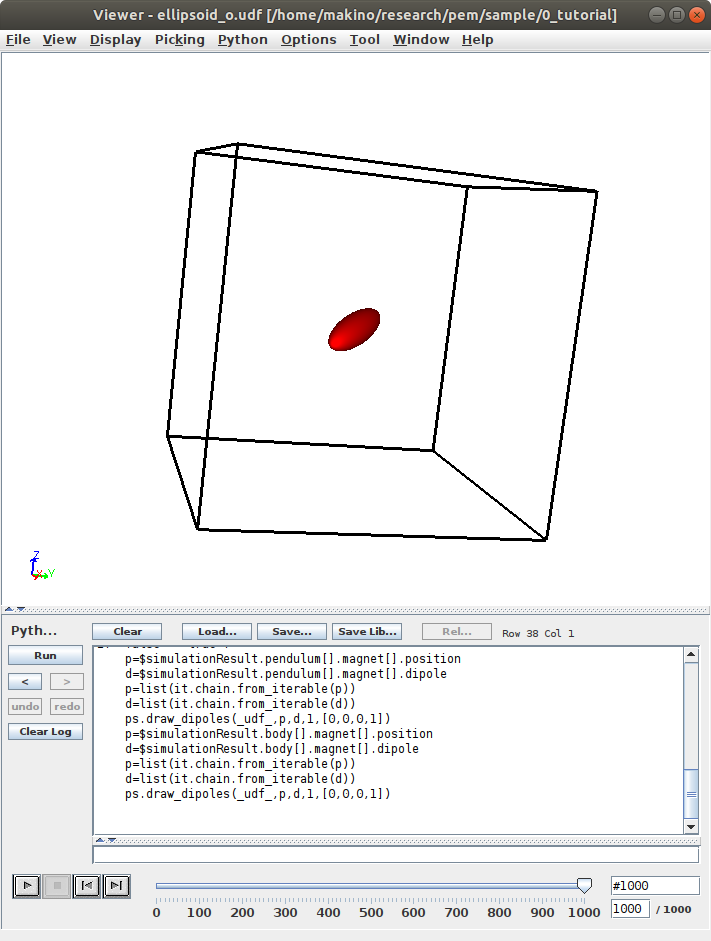
\includegraphics[clip,width=0.7\linewidth]{ellipsoid.png}
  \caption{楕円体の自由回転の描画
  }
  \label{fig:ellipsoid}
\end{figure}
gourmettermから
\begin{verbatim}
pem -I elllipsoid.udf -O ellipsoid_o.udf
\end{verbatim}
のように作成した入力ファイルと出力ファイルを指定して、実行する。
出力ファイルを設定しなければ、入力ファイルに結果が出力される。

計算した
\begin{verbatim}
ellipsoid_o.udf
\end{verbatim}
をGOURMETから開く。
データ名
\begin{verbatim}
simulationResult
\end{verbatim}
を右クリックして、
\begin{verbatim}
show...
\end{verbatim}
で、シミュレーション結果を描画できる。
適当な視点で、動画を見ることが出来る。

\section{磁石振り子}
文献\cite{doi}の152ページにある磁石振り子をシミュレーションする。
この文献のシミュレーションの枠組みでは、図\ref{fig:pendulum}(a)のように、振り子の軸のまわりに対称である必要があるが、PEMでは、図\ref{fig:pendulum}(b)のように対称である必要ない。
\begin{figure}[h]
\centering
  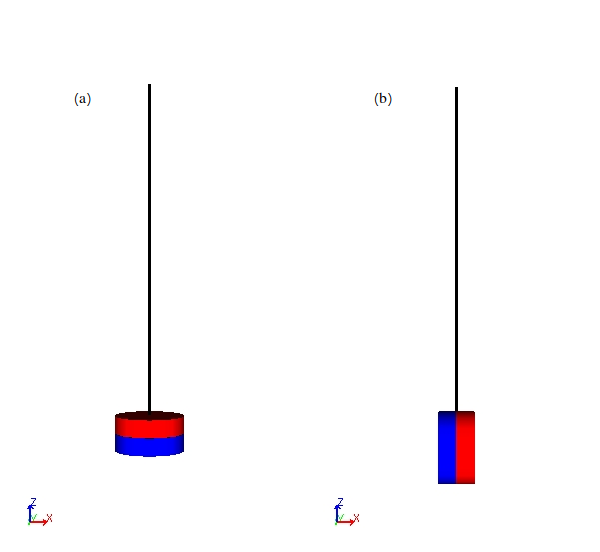
\includegraphics[clip,width=0.7\linewidth]{pendulum.png}
  \caption{振り子の例。(a)は軸のまわりで対称。(b)は非対称な場合。
  }
  \label{fig:pendulum}
\end{figure}
\begin{figure}[h]
\centering
  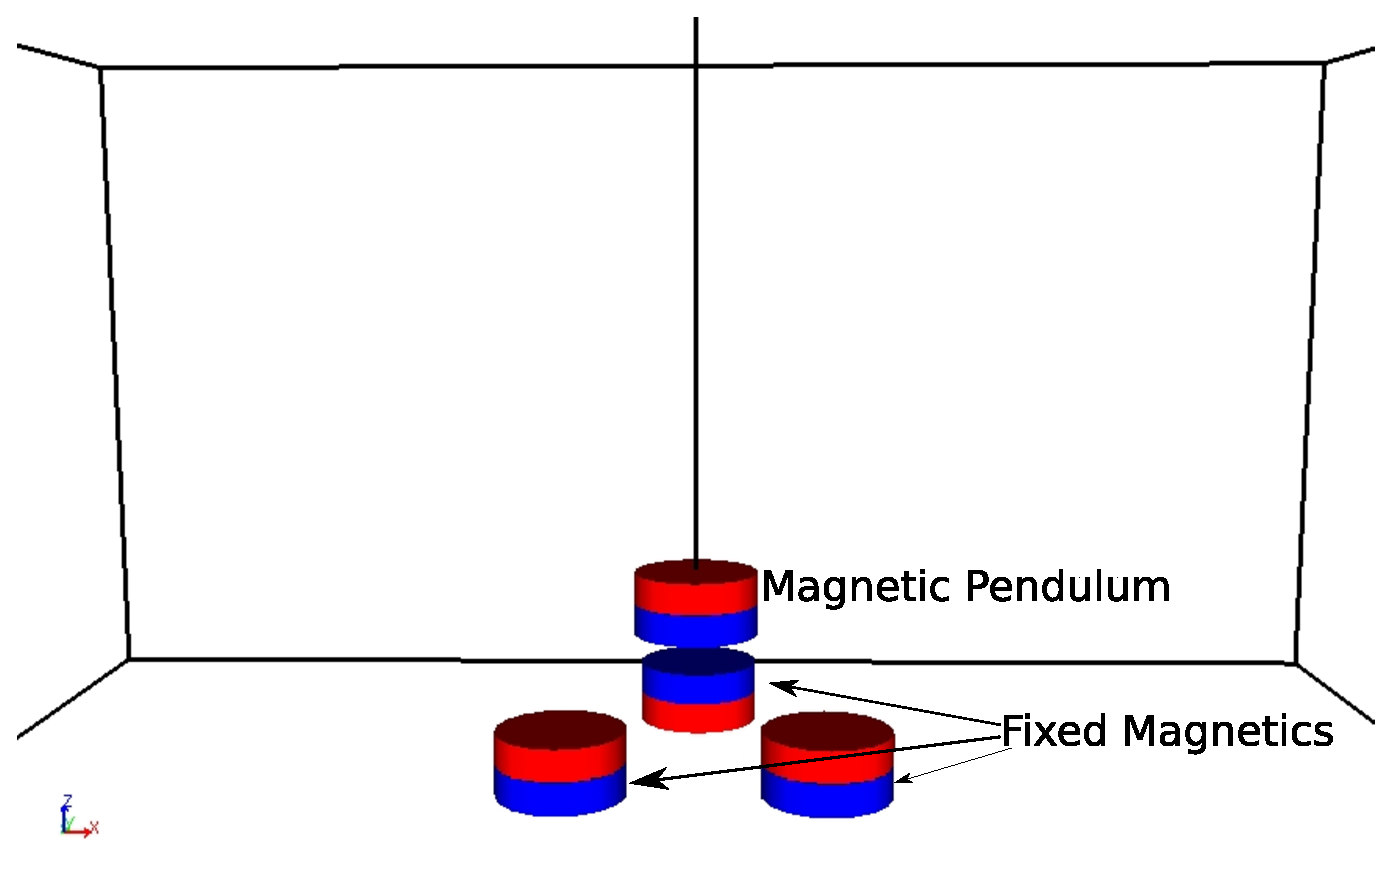
\includegraphics[clip,width=0.7\linewidth]{magneticPendulum.eps}
  \caption{磁石振り子。固定された磁石があり、相互作用することにより複雑な運動をする。
  }
  \label{fig:magneticPendulum}
\end{figure}
\subsection{入力UDF}
図\ref{fig:magneticPendulum}は、目標とするシミュレーションである。

赤色を磁石のN極、青色をS極として描画している。
磁石の振り子があり、下に固定された磁石と相互作用することにより、振り子は複雑な運動をする。

ここでは、
\begin{verbatim}
body[0]
body[1]
\end{verbatim}
と2つ設定する。
片方が、振り子で、片方が下に設置する磁石である。
まず磁石の振り子を
\begin{verbatim}
body[0]
\end{verbatim}
に設定する。
\begin{verbatim}
body[0].shape[0]
body[0].shape[1]
\end{verbatim}
に円筒で色を変えてN極とS極を表現している。
粒子固定座標系の原点が回転中心なので、円筒の長さを考えて、配置している。
\begin{verbatim}
body[0].shape[22]
\end{verbatim}
は描画用に、直線を設定している。質量がゼロであるから、物理的には意味をなさない。

\begin{verbatim}
body[0].magnet[0]
\end{verbatim}
には、振り子の磁石を設定している。

\begin{verbatim}
body[1]
\end{verbatim}
では、下に固定する磁石の形状を設定している。
\verb|body[0]|のものと似てはいえるが、振り子の軸の部分がなく、原点に磁石の中心がある。

\begin{verbatim}
simulation.pendulum[0]
\end{verbatim}
に、振り子を設定する。回転中心を実験室系の原点においている。
初期速度を\verb|simulation.pendulum[0].angularVelocity|に設定して運動するようにしている。
\begin{verbatim}
simulation.body[0]
simulation.body[1]
simulation.body[2]
\end{verbatim}
で磁石を設定している。
特に
\begin{verbatim}
simulation.body[0].orientation
\end{verbatim}
は\verb|simulation.body[0].orientation.u3.z|を\verb|-1|として、磁石を反転している。
また、右手系を保つために
\verb|simulation.body[0].orientation.u2.y|も\verb|-1|にしている。

\begin{verbatim}
simulation.gravity
\end{verbatim}
に重力を設定して、入力udfが出来た。

\subsection{シミュレーションの実行、結果}

gourmettermから
\begin{verbatim}
pem -I magnetic_pendulum.udf -O magnetic_pendulum_o.udf
\end{verbatim}
のように実行。
出力されるファイルをGOURMETで開いてアニメーションを見ると、複雑な運動をしているのが分かる。
例えば、下のpythonをgourmettermから実行すると図\ref{fig:trajectory}のように軌跡が分かる。ただしmatplotlibをpipでインストールしておく必要がある。

\begin{verbatim}
import numpy as np
from UDFManager import UDFManager
import matplotlib.pyplot as plt
from mpl_toolkits.mplot3d import Axes3D

udf=UDFManager("pendulum_o.udf")
pos=[]
n=udf.totalRecord()
for i in range(n):
    udf.jump(i)
    p=np.array(udf.get("simulationResult.pendulum[0].magnet[0].position"))
    pos.append(p)
pos=np.array(pos)
#
fig = plt.figure(figsize=(9,5))
ax = fig.add_subplot(111, projection='3d')
ax.plot(pos[:,0],pos[:,1],pos[:,2],color="blue")
ax.scatter(pos[::10,0],pos[::10,1],pos[::10,2],color="black")
ax.set_xlabel("X")
ax.set_ylabel("Y")
ax.set_zlabel("Z")
ax.set_xlim(-4,4)
ax.set_ylim(-4,4)
ax.set_zlim(-12,2)
ax.set_title("Bob trajectory")
#
plt.tight_layout()
plt.savefig('./trajctory.png')
plt.show()
\end{verbatim}

\begin{figure}[h]
\centering
  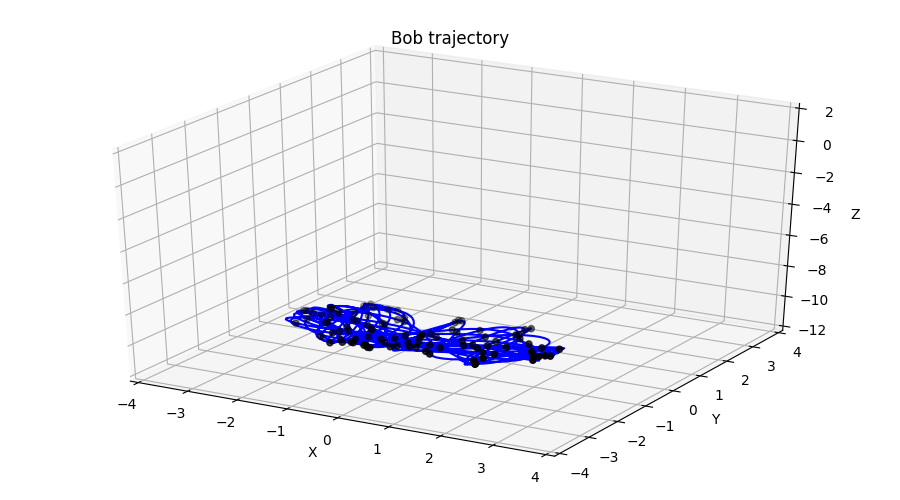
\includegraphics[clip,width=0.7\linewidth]{trajectory.png}
  \caption{磁石振り子の磁石の位置の軌跡
  }
  \label{fig:trajectory}
\end{figure}

たとえば、磁石の向きを変えたものが、
\begin{verbatim}
magnetic_pendulum2.udf
\end{verbatim}
である。振り子の軸で対称でない場合もシミュレーションできる。

実際の実験では、摩擦があるため、最終的に振り子は、どこかで止まってしまう。
udfの
\begin{verbatim}
simulation.PseudoFrictionTorque
\end{verbatim}
を有効にしているのが、
\begin{verbatim}
magnetic_pendulum_friction.udf
\end{verbatim}
である。
十分に時間が経った結果、図\ref{fig:pendulum_equlibrium}に、N極とS極とが引き合う位置が平行位置として計算されており、
最終的な位置は、適切と考えられる。
しかし、摩擦が振り子の向きに関係なく等方的な摩擦が入っているなど、動力学には、妥当性はない。
\begin{figure}[h]
\centering
  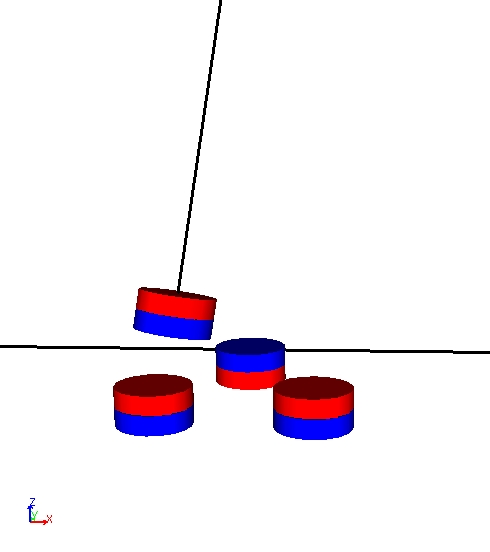
\includegraphics[clip,width=0.6\linewidth]{pendulum_equlibrium.jpg}
  \caption{平衡時の振り子の位置
  }
  \label{fig:pendulum_equlibrium}
\end{figure}

\begin{thebibliography}{9}
  \bibitem{doi}土井正男、滝本淳一編   物理仮想実験室 名古屋大学出版  (2004)
\end{thebibliography}
\end{document}